\chapter{Anwendung statistischer Methoden}

In diesem Kapitel werden nun mehrere Programmiersprachen vorgestellt, die sich für Regressionsanalyse eignen. Im letzten Teilkapitel wird demonstriert, wie man solche Methoden mit vorhandener SQL-Syntax umsetzen und durchführen kann.

\section{Beispieldaten}

Um Regressionsanalyse auch praktisch betreiben zu können, arbeiten wir in dieser Arbeit mit einem Satz an Beispieldaten. Diese Daten wurden mit einem Python-Skript erstellt, welches im als Ganzes im Anhang zu finden ist. Dabei werden die einzelnen Merkmale eines Datensatzes mit Absicht so erstellt, dass eine Korrelation zwischen diesen bewusst erzeugt oder nicht erzeugt wird. Diese Beispieldaten liegen in Form einer csv-Datei vor, welche in jeder Sprache einfach eingelesen werden kann.

Wir betrachten hier fiktive Kunden von Amazon. Für jeden Kunden wissen wir das Alter, die Anzahl seiner Käufe, die Summe des ausgegebenen Geldes und ob der Kunde Amazon-Prime Mitglied ist oder nicht. Der ausgegebene Betrag wird in Cent angegeben, um mit ganzen Zahlen rechnen zu können. Die Prime-Mitgliedschaft wird mit einer 1 symbolisiert, während eine 0 das Gegenteil bedeutet.

Insgesamt wurden für diese Arbeit 100.000 solcher Datensätze erzeugt. In der folgenden Tabelle sind die ersten 10 Datensätze beispielhaft dargestellt.

\begin{center}
  \begin{tabular}{|c|c|c|c|}\hline
    \textbf{age} & \textbf{purchases} & \textbf{money} & \textbf{prime} \\ \hline
    30 & 1 & 4421 & 0 \\ \hline
    30 & 11 & 23346 & 1 \\ \hline
    33 & 1 & 4010 & 0 \\ \hline
    31 & 19 & 52517 & 1 \\ \hline
    29 & 3 & 8046 & 0 \\ \hline
    28 & 12 & 25295 & 0 \\ \hline
    41 & 16 & 38236 & 1 \\ \hline
    23 & 3 & 7098 & 1 \\ \hline
    25 & 1 & 2707 & 0 \\ \hline
    38 & 20 & 50976 & 1 \\ \hline
  \end{tabular}
\end{center}

Wir definieren uns außerdem drei Fragestellungen, welche wir jeweils mit einer Art der in Kapitel 2 vorgestellten Regressionen beantworten werden:
\begin{enumerate}
  \item Zuerst wollen wir wissen, ob das ausgegebene Geld mit der Anzahl der Käufe in linearem Zusammenhang steht. Diese Fragen können wir mit einfacher linearer Regression beantworten. $money$ ist hierbei die abhängige Variable und $purchases$ ist die unabhängige Variable.
  \item Die zweite Frage ist ähnlich der ersten, nur wollen wir hier wissen, ob neben der Anzahl der Käufe auch das Alter des Kunden einen linearen Einfluss auf das ausgegebene Geld hat. Hier haben wir nun zwei unabhängige Variablen, nämhlich $age$ und $purchases$. Die abhängige Variable bleibt $money$. Diese Frage beantworten wir also mit multipler linearer Regression.
  \item Als letztes interessiert uns, ob eine Prime-Mitgliedschaft von der Summe des ausgegebenen Geldes zusammenhängt. $money$ ist also nun die unabhängige Variable, während $prime$ die abhängige Variable ist. Außerdem ist $prime$ eine binäre Variable. Deshalb nutzen wir hier also logistische Regression.
\end{enumerate}

\section{R-Projekt}
Das R-Projekt oder einfach nur R ist eine Sprache für statistische Berechnungen und graphische Darstellung. Damit ist R wie geschaffen für Regressionsanalyse. Von allen hier behandelten Sprachen ist R damit auch die einfachste und direkteste für Regression.

\subsection{Grundprinzip}

In R sind einfache Datenstrukturen wie Vektoren, Matrizen und Listen als Datentypen vorhanden. Darauf aufbauend existieren sogenannten Dataframes. Ein Dataframe ist eine Liste von Vektoren der gleichen Länge und wird in R zur Repräsentation von Datentabellen verwendet. Die Vektoren der Liste entsprechen dann den Spalten der Tabelle. In einen solchen Dataframe importieren wir unsere Daten.

In R lassen sich außerdem sehr einfach sogenannte Modelle definieren, welche als Eingabe nur die Daten und eine Formel benötigen. Eine Formel ist von der Form $y \sim modell$ und enthält den funktionalen Zusammenhang zwischen der abhängigen und den unabhängigen Variablen.

Hat man ein Modell erstellt, so bietet R einfache Funktionen, um die Parameter für das gegebene Modell mittels Regressionsanalyse zu berechnen. Wir werden im Folgenden von den Funktionen $lm$ (für "linear model") und $glm$ für ("generalized linear model") Gebrauch machen.

\subsection{Einfache lineare Regression}

Betrachten wir also Frage Nummer $1$ aus dem vorherigen Teilkapitel. Die Formel lautet dann einfach $money \sim purchases$. Man liest also die Daten aus der csv-Datei, erstellt das Modell mit der genannten Formel und berechnet die Parameter mit der Funktion $lm$. Insgesamt braucht man also nur drei Zeilen Code. Die print-Funktion dient hierbei nur zur Ausgabe des Ergebnisses.

\begin{minted}[linenos,breaklines,frame=single]{r}
  data <- read.csv2("sample.csv", sep = ",", header = TRUE)
  modell <- as.formula("money ~ purchases")
  slr <- lm(modell, data = data)
  print(slr)
\end{minted}

Das Ergebnis des obigen Codes ist folgendes:

\begin{minted}[linenos,breaklines,frame=single]{r}
  Coefficients:
  (Intercept)    purchases
        1.941     2500.805
\end{minted}

Der Wert unter $(Intercept)$ entspricht dabei dem Paramter $\alpha$ in unserer Notation, der Wert unter $purchases$ entspricht $\beta$.

Wir wollen dieses Ergebnis kurz interpretieren. Der kleine Wert für $\alpha$ entspricht der Intuition, dass ein Kunde ohne Käufe auch kein Geld ausgegeben hat. Der relativ große Wert von ca. $2500$ für $\beta$ zeigt, dass die Anzahl der gekauften Artikel sehr einen großen Einfluss auf das ausgegebene Geld hat. Die Kunden geben pro gekauftem Artikel etwa $2500$ Cent, also $25$ Euro aus.

R verfügt auch über Möglichkeiten zur graphischen Darstellung. Lässt man die die Datenpunkte und die lineare Ausgleichsfunktion mit den berechneten Parameter plotten, erhält man dieses Ergebnis:

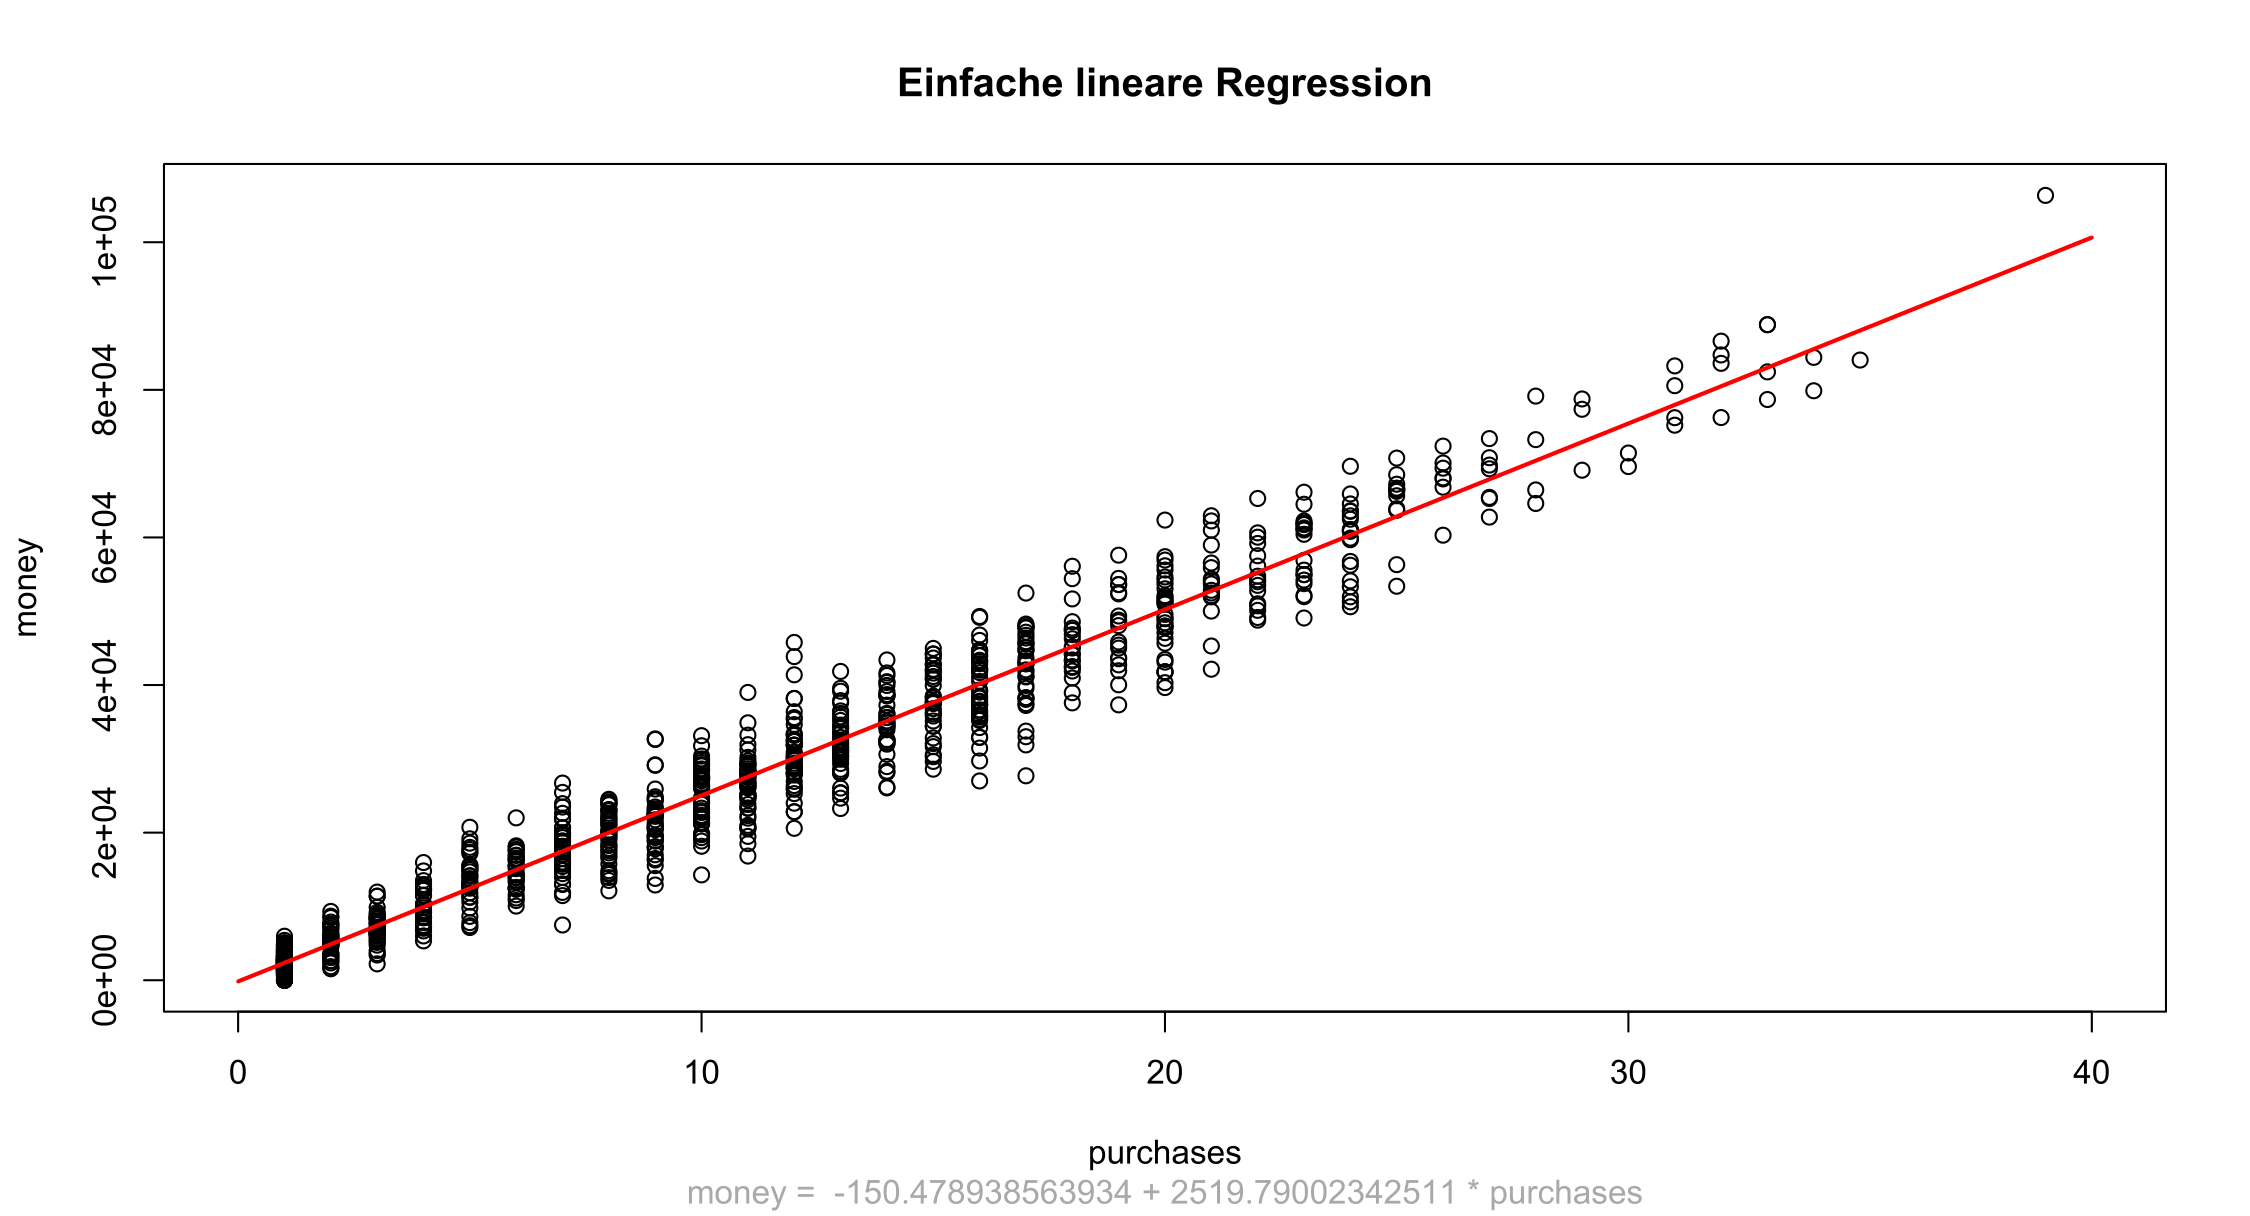
\includegraphics[width=\textwidth]{r-simpleLinearRegression}

\subsection{Multiple lineare Regression}

Bei multipler lineare Regression unterscheidet sich der R-Code nur in der Wahl der Formel. Hier wollen wir $money$ durch eine lineare Summe von $purchases$ und $age$ modellieren, deshalb lautet die Formel hier $money \sim purchases + age$. Man erhält das folgende Ergebnis.

\begin{minted}[linenos,breaklines,frame=single]{r}
  Coefficients:
  (Intercept)    purchases          age
     -16.4842    2500.8042       0.5318
\end{minted}

Auch hier eine kurze Interpretation dieses Ergebnisses: Der Wert für $\alpha$ ist wieder relativ klein, der Wert für das $\beta$ zu $purchases$ ist fast exakt derselbe wie bei einfacher linerarer Regression, was bei denselben Daten auch zu erwarten war. Der Wert für das $\beta$ zu $age$ ist dagegen nahe bei null. Das bedeutet, dass das Alter neben der Anzahl der Käufe keinen signifikanten Einfluss auf das ausgegebene Geld hat.

\subsection{Logistische Regression}

Bei logistischer Regression nutzen wir nun nicht mehr ein lineares Modell wie bisher, sondern ein generalisiertes lineares Modell. Logistische Regression ist im Wesentlichen ein Spezialfall dieses Modelles. Hier nutzen wir also die $glm$-Funktion. Um logistische Regression damit betreiben zu können, wählt man den Parameter $family$ dieser Funktion als $binomial$.

Man braucht wie auch bei linearer Regression ein Formel für das Modell. Diese bildet man analog wie bisher, indem mal die abhängige Variable mit den unabhängigen Variablen über eine Tilde verbindet. Im Fall der dritten Fragestellung aus Kapitel 3.1 wählen die also die Formel $prime \sim money$.

Der gesamte R-Code für die logistische Regression lautet also wiefolgt:

\begin{minted}[linenos,breaklines,frame=single]{r}
  data <- read.csv2("sample.csv", sep = ",", header = TRUE)
  modell <- as.formula("prime ~ money")
  logit <- glm(modell, family = binomial, data = data)
  print(logit)
\end{minted}

Nach der Ausführung erhält man das folgende Ergebnis:

\begin{minted}[linenos,breaklines,frame=single]{r}
  Coefficients:
  (Intercept)        money
  -1.9145608    0.0000769

  Degrees of Freedom: 99999 Total (i.e. Null);  99998 Residual
  Null Deviance:	    138600
  Residual Deviance: 100500 	AIC: 100500
\end{minted}

Eine anschauliche Interpretation der zurückgegebenen Parameter ist nicht mehr so einfach. Wir lassen uns das Ergebnis daher wieder als Plot visualisieren:

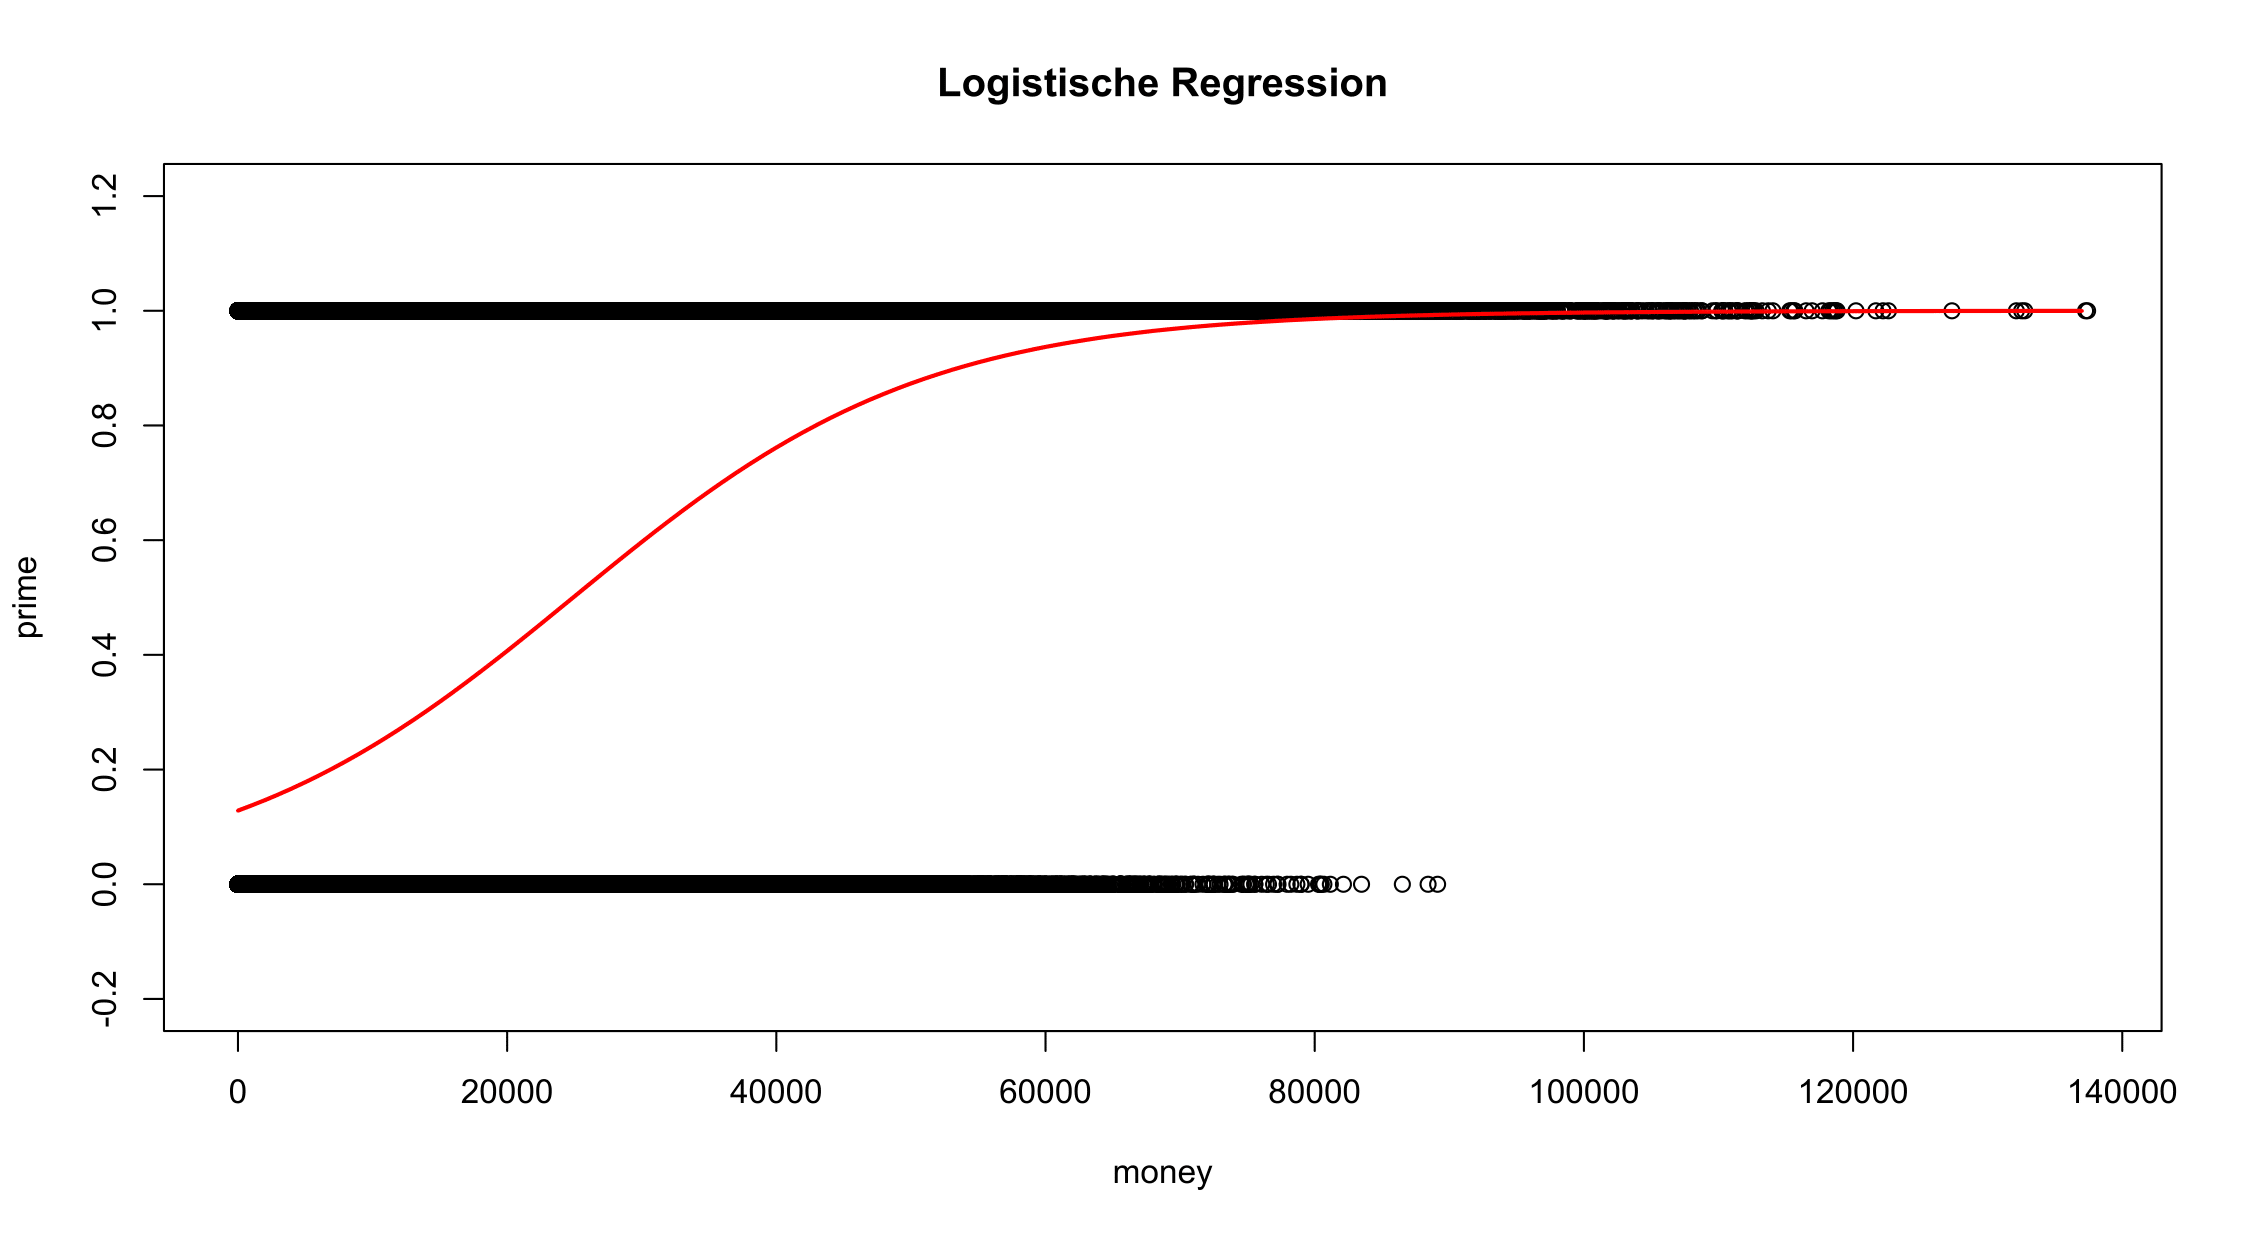
\includegraphics[width=\textwidth]{r-logisticRegression}

Für Kunden, die weniger als $100$ Euro ausgegeben haben ist die Wahrscheinlichkeit Prime-Mitglied zu sein mit etwa $25\%$ relativ gering. Je höher die Summe aber wird, desto größer wird auch diese Wahrscheinlichkeit. So ist ein Kunde mit mehr als $800$ Euro Ausgaben so gut wie immer ein Prime-Mitglied.

\section{TensorFlow}

TensorFlow ist eine Software-Bibliothek, die unter der Haube von Google für die Umsetzung von Algorithmen für maschinelles Lernen entwickelt wurde. Das umfasst insbesondere auch die Möglichkeit zur iterativen Optimierung von Kostenfunktionen, was wir nun für Regressionsanalyse nutzen wollen.

TensorFlow bietet APIs für verschiedene Programmiersprachen an. Die Skripte, welche für dieser Arbeit erstellt wurden, sind in Python geschrieben. Im Unterschied zu den Ergebnissen der R-Skripte werden wir hier nicht dieselben Ergebnisse erhalten. Wir verwenden TensorFlows Implementierung eines Gradientenabstiegsverfahrens, für welches man die Anzahl der Schritte und die Abstiegsgeschwindigkeit selbst wählen muss. Die Genauigkeit der berechneten Parameter hängt also zusätzlich von einer angemessenen Auswahl dieser Werte ab.

Die Python-Skripte umfassen nun zwischen 70 und 100 Codezeilen, daher findet man diese Skripte im Ganzen nur im Anhang. Die wichsten Ausschnitte sollen im folgenden aber einen Einblick in die Funktioneweise des Codes geben.

\subsection{Grundprinzip}

TensorFlow arbeitet auf dem untersten Level mit Tensoren. Das sind im Wesentlichen Matrizen mit festen Dimensionen. Diese Tensoren können dann mit Hilfe aller möglicher Operatoren weiterverarbeitet werden.

Es gibt drei Möglichkeiten, Tensoren zu definieren: Als Konstante, als Variable oder als Platzhalter. Während Konstanten ihren Wert nicht mehr ändern können, sind die beiden letztgenannten veränderbar. Der Unterschied besteht darin, dass Variablen mit einem Startwert initiiert werden und Platzhalter ohne Wert. Wir werden Variablen nutzen, um die Parameter über die Iterationen zu speichern. Die Daten, mit denen wir das Modell trainieren werden, übergeben wir an Platzhalter.

Wie das Modell exakt definiert wird zeigen die folgenden Teilkapitel. Allgemein gesamt wird eine Kostenfunktion aufgestellt, die dann mit Hilfe eines Gradientenabstiegsverfahrens iterativ minimiert wird. Die Definition dieses sogenannten Trainingsschrittes sieht immer gleich aus:

\begin{minted}[linenos,breaklines,frame=single]{python}
  train_step = tf.train
                 .GradientDescentOptimizer(learn_rate)
                 .minimize(cost)
\end{minted}

Dabei ist $tf$ die importierte TensorFlow-Bibliothek, $learn\_rate$ ist die Geschwindigkeit bzw. Schrittweite des Verfahrens und $cost$ ist die zuvor definierte Kostenfunktion.

Um dann auch wirklich Berechnungen durchführen zu können, muss in TensorFlow eine Session erzeugt werden. In dieser Session wird dann die Iteration gestartet, die $train_step$ immer wieder mit echten Daten füttert. Je mehr Iterationen, desto exakter werden die Parameter.

\subsection{Einfache lineare Regression}

Hier definieren wir unsere Platzhalter und Variable wiefolgt:

\begin{minted}[linenos,breaklines,frame=single]{python}
  x = tf.placeholder(tf.float32, [None, 1])
  y = tf.placeholder(tf.float32, [None, 1])
  alpha = tf.Variable(tf.zeros([1]))
  beta = tf.Variable(tf.zeros([1, 1]))
\end{minted}

$x$ und $y$ sind die Platzhalter der wahren Werte für das folgende Training. $alpha$ und $beta$ sind die Parameter-Variablen, welche mit null-Werten initiiert werden. Daraus berechnen wir über den linearen funktionalen Zusammenhang die geschätzten $y$ Werte:

\begin{minted}[linenos,breaklines,frame=single]{python}
  y_calc = tf.matmul(x, beta) + alpha
\end{minted}

Die Funktion $matmul$ führt Matrizenmultiplikation durch. Nun definieren wir noch die Kostenfunktion als Mittelwert der Quadrate zwischen den wahren und berechneten $y$-Werten:

\begin{minted}[linenos,breaklines,frame=single]{python}
  cost = tf.reduce_mean(tf.square(y - y_calc))
\end{minted}

Damit können wir die Session starten und unsere Parameter berechnen lassen. Mit einer Schrittweite von $0.0054$ und $2000$ Iterationen erhält man folgendes Ergebnis:

\begin{minted}[linenos,breaklines,frame=single]{python}
  alpha:  1.976688
  beta:   2500.802979
  cost:   13818006.000000
\end{minted}

Die Werte für $alpha$ und $beta$ sind damit schon sehr nahe an den exakten Werten. Zusätzlich wird hier auch der aktuelle Wert für die Kostenfunktion ausgegeben.

\subsection{Multiple lineare Regression}

Nachdem in diesem Fall nun mehr unabhängige Variablen vorhanden sind, vergrößern wir die Größe der Tensoren $x$ und $beta$ um eins.

\begin{minted}[linenos,breaklines,frame=single]{python}
  x = tf.placeholder(tf.float32, [None, 2])
  beta = tf.Variable(tf.zeros([2, 1]))
\end{minted}

Die restlichen Variablen werden wie bei einfacher linearer Regression definiert. Das Gradientenverfahren ist bei zwei abhängigen Variablen ineffizienter und komplexer, daher muss die Schrittweite verringert werden. Eine Folge davon ist, dass man mehr Schritte für dieselbe Präzision des Ergebnisses durchführen muss. Bei einer Schrittweite von $0.00071$ und $50000$ Schritten erhält man folgendes Ergebnis:

\begin{minted}[linenos,breaklines,frame=single]{python}
  alpha:           -16.035418
  beta_purchases:  2500.799316
  beta_age:        0.521137
  cost:            13817990.000000
\end{minted}

\subsection{Logistische Regression}

Wir definieren nun unsere Tensoren wieder exakt wie bei der einfachen linearen Regression, da wie hier wieder mit je einer unabhängigen und einer abhängigen Variablen arbeiten. Die bisher verwendete Berechnung der $y$-Werte fügen wir nun zusätzlich in die logistische Funktion ein:

\begin{minted}[linenos,breaklines,frame=single]{python}
  y_calc = 1 / (1 + tf.exp(- tf.matmul(x, beta) - alpha))
\end{minted}

Die Kostenfunktion ist nun nicht mehr die Summe der Quadrate sondern im Wesentlichen die Likelihoodfunktion. TensorFlow bietet nur eine API für Minimierung, während wir hier eine Funktion maximieren wollen. Deshalb verwenden wir das Inverse der Likelihoodfunktion als Kostenfunktion. Zusätzlich wenden wir wieder einen Logarithmus auf die Funktion an:

\begin{minted}[linenos,breaklines,frame=single]{python}
  cost = - tf.reduce_sum(
    tf.log(
      y * y_calc +
      (1 - y) * (1 - y_calc)
    )
  )
\end{minted}

Wir wählen eine Schrittweite von $0.0001$ und iterieren $1000$ Schritte, um das folgende Ergebnis zu erhalten:

\begin{minted}[linenos,breaklines,frame=single]{python}
  alpha:  -1.914557
  beta:   0.000077
  cost:   50272.593750
\end{minted}

\section{SQL}

Die "Structured Query Language" alias "SQL" ist eine Sprache zur Definition und Verarbeitung von Datenstrukturen in Datenbanksystemen und wird in nahezu allen Implementierungen relationaler Datenbanken unterstützt. Of liegen die Daten, welche man für Regressionsanalyse verwenden möchte in einer solchen Datenbank.

Natürliche Methoden für Regression gehören nicht zum Portfolie von SQL, da Statistik und Datenanalyse nicht der primäre Einsatzzweck für SQL ist. Doch auch wenn jede Datenbank ihren eigenen SQL-Dialekt anbietet, ist es in nahezu allen Systemen möglch, mit standardisierten SQL-Methoden Regression direkt in der Datenbank zu betreiben.

In diesem Kapitel soll das nun für zwei der beliebtesten Open-Source-Datenbanksystemen umgesetzt werden, nämlich MySQL und PostgreSQL. Der vollständige SQL-Code befindet sich wegen der Länge wieder komplett im Anhang.

Im Gegensatz zu den beiden bisher vorgestellten Sprachen verfolgen wir hier kein Grundprinzip, in dem sich alle Regressionen ähnlich sind. Die einzige Gemeinsamkeit ist, dass wir in allen SQL-Skripten Prozeduren bzw. Funktionen definieren, welche bei Aufruf die Regressionsanalyse durchführen. Wir nehmen dazu an, dass die Daten für die Regression in einer Tabelle namens $sample$ liegen.

Bei einfacher linearer Regression berechnen wir die Parameter exakt über die Formeln aus Kapitel 2.1.1. Bei multipler Regression verwenden wir die Matrixformel aus Kapitel 2.1.2. Hier müssen wir zusätzlich Algorithmen zur Multiplikation und Invertierung von Matrizen implementieren. Für logistische implementieren wir dann ein Gradientenverfahren.

\subsection{Einfache lineare Regression}

Einfache lineare Regression stellt uns in SQL noch vor wenig Herausforderungen. Wir berechnen zuerst die Mittelwerte über die Spalten $purchases$ und $money$, dann die Summen in Zähler und Nenner der Formel für $\beta$ und können dann mit einfachen Rechenoperationen die beiden Paramter bestimmen.

Diese Berechnung kann man sogar in einer einzelnen Abfrage umsetzen. Das Skript für PostgreSQL tut das auch und definiert die genannten Berechnungsschritte als einzelne Views. In MySQL existiert die VIEW-Syntax nicht. Deshalb wird die Berechnung der Übersicht halber auf mehrere Abfragen aufgeteilt.

Führen wir die Prozeduren im jeweiligen Datenbanksystem aus, erhalten wir folgende Ergebnisse:

\begin{center}
  \captionof{table}{Einfache lineare Regression in MySQL}
  \begin{tabular}{|c|c|}\hline
    \textbf{variable} & \textbf{value} \\ \hline
    alpha & 1.94097291465000744000 \\ \hline
    beta & 2500.80479741553200000000 \\ \hline
  \end{tabular}

  \captionof{table}{Einfache lineare Regression in PostgreSQL}
  \begin{tabular}{|c|c|}\hline
    \textbf{variable} & \textbf{value} \\ \hline
    alpha & 1.94097291212994333830395091244619200000000000 \\ \hline
    beta & 2500.8047974157705841434285987976 \\ \hline
  \end{tabular}
\end{center}

\subsection{Multiple lineare Regression}

Wir wollen zur Lösung dieses Regressionsproblems die Matrix-Formel aus Kapitel 2.1.2 anwenden. Dazu müssen Methoden für das Transponieren, Multiplizieren und Invertieren von Matrizen implementiert werden, da weder MySQL noch PostgreSQL über diese Funktionen verfügt. Dazu müssen wir außerdem einen Weg finden, Matrizen im jeweiligen Datenbanksystem zu repräsentieren.

Diese Repräsentation lösen wir unterschiedlich in den beiden Datenbanksystemen. Beginnen wir mit MySQL. Hier definieren wir uns temporäre Tabellen, welche jeweils eine Matrix repräsentieren. Jede solche Tabelle besteht aus drei Spalten, nämlich $row$, $column$ und $value$. Die ersten beiden enthalten die Indizes des Matrixelements, letztere enthält den Wert des jeweiligen Elements.

Wir definieren insgesamt sieben solcher Tabellen:
\begin{itemize}
  \item $matrix\_X$: Entspricht der Matrix $X$ aus der Berechnungsformel.
  \item $matrix\_y$: Entspricht der Matrix $y$ aus der Berechnungsformel.
  \item $matrix\_transposed$: Entspricht der Matrix $X^T$.
  \item $matrix\_product\_1$: Entspricht dem Matrixprodukt $X^t X$.
  \item $matrix\_inverse$: Entspricht dem Inversen des obigen Matrixprodukts $(X^T X)^{-1}$.
  \item $matrix\_product\_2$: Entspricht dem Matrixprodukt $X^T y$.
  \item $matrix\_result$: Entspricht dem Endergebnis der Berechnungsformel $(X^T X)^{-1} X^T y$.
\end{itemize}

Die ersten beiden dieser Tabellen werden einfach mit den vorhandenen Werten aus der Tabelle $sample$ befüllt. Die Tabelle $matrix\_transposed$ wird mit einem einfachen Query aus der Tabelle $matrix_X$ berechnet, indem die Indizes für Zeile und Spalte vertauscht werden.

Die Tabellen $matrix\_product\_1$, $matrix\_product\_2$ und $matrix\_result$ sind Ergebnisse von Matrizenmultiplikationen. Diese Produkte werden mit zwei Schleifen berechnet, die über die Zeilen und Spalten der Ergebnismatrix iterieren. Jeden Element der zu berechnenden Matrix wird dann über eine Abfrage berechnet, welche die jeweilige Zeile und Spalte der beiden Faktor-Tabellen zusammenjoint und über das Ergebnis summiert. Die Abfrage fügt das Ergebnis der Summierung in die Zieltabelle ein.

Bei den Tabellen $matrix\_product\_2$ und $matrix\_result$ ist die eine Dimension der zu berechnenden Tabelle gleich eins ist. Die zweite Schleife besitzt also eine Iteration, weswegen diese in dem SQL-Skript auch einfach weggelassen wird.

Für die Berechnung der inversen Matrix, also für die Tabelle $matrix\_inverse$ wird ein einfacher iterativer Algorithmus verwendet, welcher über alle Zeilen der zu invertierenden Matrix läuft. In jedem Schritt werden alle Elemente der Matrix nach einem bestimmten Schema angepasst. Details zu dem verwendeten Algorithmus findet man in \cite{matrix}.

Die komplette Berechnung wurde in eine Prozedur verpackt. Führt man diese aus, erhält man das folgende Ergebnis:

\begin{center}
  \captionof{table}{Multiple lineare Regression in MySQL}
  \begin{tabular}{|c|c|}\hline
    \textbf{variable} & \textbf{value} \\ \hline
    alpha & -16.48419722318438785193 \\ \hline
    beta\_purchases & 2500.80422198935324307395 \\ \hline
    beta\_age & 0.53177717855855479093 \\ \hline
  \end{tabular}
\end{center}

Betrachten wir nun die Implementierung in PostgreSQL. Gegenüber MySQL hat man hier den Vorteil, dass mehrdimensionale Listen als Datentyp existieren. Wir brauchen nun also keine temporären Tabellen für die Matrizen mehr, sondern speichern diese einfach als zweidimensionales Array vom Datentyp $NUMERIC$.

Neben der eigentlichen Prozedur zum Ausführen der Regression definieren wir drei weitere Funktionen:
\begin{itemize}
  \item $matrix\_transpose$: Diese Funktion nimmt ein zweidimensionales Array von Typ $NUMERIC$ als Input und gibt die transponierte Matrix zurück. Die Transponierte wird mit zwei Schleifen über die Zeilen und Spalten gebildet, welche im Wesentlichen die Zeilen- und Spaltenindizes vertauschen.
  \item $matrix\_multiplication$: Diese Funktion nimmt zwei zweidimensionale Arrays vom Typ $NUMERIC$ als Input und gibt das Produkt der beiden Matrizen zurück. Hier werden drei Schleifen zur Berechnung verwendet. Die ersten beiden iterieren über die Zeilen und Spalten der Ausgabematrix. Die dritte iteriert über die Zeile bzw. Spalte, welche zur Berechnung der aktuellen Elements verwendet werden und addiert die Produkte der Elemente dieser Zeile und Spalte auf.
  \item $matrix\_inversion$: Diese Funktion nimmt ein zweidimensionales Array vom Typ $NUMERIC$ als Input und gibt das Inverse dieser Matrix zurück. Dabei wird derselbe Algorithmus verwendet, der auch in MySQL implementiert wurde.
\end{itemize}

Mit diesen drei Funktionen lässt sich die Formel aus Kapitel 2.1.2 mit drei Abfragen umsetzen. Dazu erzeugen wir zuerst zwei Matrizen $x$ und $y$ mit den unabhängigen und der abhängigen Variable als Elemente aus der $sample$-Tabelle. Im dritten Query nutzen wir die genannten Funktionen, um die Matrix mit den gesuchten Parametern zu berechnen.

Führt man die multiple lineare Regressionsanalyse in PostgreSQL durch, erhält man das folgende Ergebnis:

\begin{center}
  \captionof{table}{Multiple lineare Regression in PostgreSQL}
  \begin{tabular}{|c|c|}\hline
    \textbf{variable} & \textbf{value} \\ \hline
    alpha & -16.48419722318438785193 \\ \hline
    beta\_purchases & 2500.80422198935324307395 \\ \hline
    beta\_age & 0.53177717855855479093 \\ \hline
  \end{tabular}
\end{center}

Da wir dieselben Algorithmen und dieselbe Präzision für Kommazahlen in MySQL und PostgreSQL verwendet haben, stimmen die beiden Ergebnisse sogar exakt überein.

\subsection{Logistische Regression}

Um logistische Regression in SQL betreiben zu können, möchten wir ein Gradientenverfahren zur Lösung implementieren. Wir implementieren denselben Algorithmus in MySQL und PostgreSQL, das heißt die Skripte unterscheiden sich lediglich in der datenbankspezifischen Syntax.

Wir verwenden für das Verfahren mehrere Tabellen, in denen wir gewissen Informationen speichern und verarbeiten werden:
\begin{itemize}
  \item Die Tabelle $datapoints$ besteht aus drei Spalten $id$, $variable$ und $value$. Die $id$-Spalte enthält einen hier generierten Wert, der einen Datensatz aus der $sample$-Tabelle identifiziert. Die $variable$-Spalte enthält den Namen der gespeicherten unabhängigen Variable. In unserem Fall steht hier immer $beta_money$, da wir nur eine unabhängige Variable betrachten. Gegebenenfalls können hier mehrere Variablen betrachtet werden. (Die Werte für einen Datenpunkt werden dann also auf mehrere Zeilen aufgeteilt.) Die Spalte $value$ enthält dann den Wert der entsprechenden Variable des jeweiligen Datensatzes.
  \item Die Tabelle $binary\_values$ besteht aus zwei Spalten $id$ und $value$. Hier werden für jeden Datenpunkt die Werte der abhängigen binären Variable gespeichert, in unserem Fall also die Werte aus der Spalte $prime$.
  \item Die Tabelle $parameters$ besteht aus drei Spalten $variable$, $old$ und $new$. Die erste Spalte enthält den Namen des Parameters, also $alpha$ oder $beta_money$. Die Spalten $old$ und $new$ enthalten die Werte der Parameter vor bzw. nach dem aktuellen Schritt im Gradientenverfahren. Wir benötigen beide Werte, um überprüfen zu können, ob die neuen Parameter ein besseres Ergebnis liefern als die alten.
  \item Die Tabelle $logits$ besteht aus drei Spalten $id$, $old$ und $new$. Hier werden für jeden Datenpunkt die Werte der logistischen Funktion $\pi_i$ berechnet. Dabei werden einmal die alten und einmal die neuen Parameter zur Berechnung verwendet.
  \item Die Tabelle $gradient$ besteht aus zwei Spalten $variable$ und $value$. Hier wird der Gradient bzw. die Werte der partiellen Ableitungen nach jedem Parameter gespeichert.
\end{itemize}

Wir definieren außerdem einige Hilfsfunktionen:
\begin{itemize}
  \item $calculate\_logits$: Diese Funktion berechnet die Werte für die logistische Funktion für alle Datenpunkte und trägt diese in die Tabelle $logit$ ein. Dabei wird die Funktion für beide Parameterwerte ($old$ und $new$) aus der Tabelle $parameters$ durchgeführt.
  \item $calculate\_gradient$: Diese Funktion berechnet den Gradienten aus Basis der alten Parameterwerte und der Werte der logistischen Funktion aus der Tabelle $logits$.
  \item $calculate\_parameters$: Diese Funktion nimmt eine Schrittweite als Argument, berechnet daraus und aus den Werten der $gradient$-Tabelle die neuen Parameter und schreibt diese zurück in die Spalte $new$ der Tabelle $parameters$.
  \item $are\_new\_parameters\_better$: Diese Funktion berechnet den Logarithmus der Likelihoodfunktion für die neuen und alten Parameter aus der Tabelle $parameters$ und gibt einen Wahrheitswert zurück. Die Rückgabe ist wahr, wenn die Likelihoodfunktion für die neuen Parameter einen größeren Wert annimmt als für die alten Parameter.
\end{itemize}

Wir führen wie schon bei TensorFlow zuerst eine Lineartransformation für die Werte aus $money$ durch und bilden diese linear auf das Interval $[0, 1]$ ab. Das dient erneut dazu, dass die Werte der logistischen Funktion nicht zu nahe an null geraten. Die transformierten Werte fügen wir in die $datapoints$-Tabelle ein. Auch die anderen Tabellen erzeugen wir und fügen initiale Werte ein. Als Anfangswert für Schrittweite wählen wir eins.

Es folgt eine $while$-Schleife, die solange läuft, bis entweder die vorgegebene Anzahl an Schritten erreicht wurde, oder die Schrittweite zu klein für die gewählte Präzision der Kommazahlen wird. Wir berechnen zuerst den Gradienten, dann die neuen Parameter. Dann ist ein Aufruf von $calculate\_logits$ nötig, um die logistische Funktion für die neuen Parameter zu berechnen.

Wir überprüfen, ob die neuen Parameter wirklich besser sind als die alten. Falls nicht, wird die Schrittweite halbiert, die Parameter und die Werte der logistischen Funktion werden erneut berechnet. Das wird solange wiederholt, bis die neuen Parameter besser sind oder die Schrittweite unter die Präzisionsgrenze fällt.

Haben wir die neuen Parameter erfolgreich berechnet, werden die Werte der $old$-Spalten in den Tabellen $parameters$ und $logits$ mit den neuen Werten überschrieben und der Iterationsschritt ist beendet. Nachdem die Schleife beendet wurde, werden die Parameter wieder entsprechend linear transformiert, um den tatsächlichen Werten für $money$ zu entsprechen.

Wir entscheiden und für 1000 Iterationen und führen die Prozeduren im jeweiligen Datenbanksystemen aus. Das Ergebnis ist folgendes:

\begin{center}
  \captionof{table}{Logistische Regression in MySQL}
  \begin{tabular}{|c|c|}\hline
    \textbf{variable} & \textbf{value} \\ \hline
    alpha & -1.914557182274162638251159505078 \\ \hline
    beta\_money & 0.000076896120535027827177415284 \\ \hline
  \end{tabular}

  \captionof{table}{Logistische Regression in PostgreSQL}
  \begin{tabular}{|c|c|}\hline
    \textbf{variable} & \textbf{value} \\ \hline
    alpha &  \\ \hline
    beta\_money &  \\ \hline
  \end{tabular}
\end{center}
